\section{Dataset \& Annotator Tool}
\label{sec:dataset}
The dataset consists of books from the 16\textsuperscript{th} and
17\textsuperscript{th} century, which were downloaded from Google Books.
\begin{comment}
%Moved to annotator part of this section
There are several peculiarities. Table
\ref{tab:statistics} shows that the amount of pages per book, and the amount of
images per book differs enormously per book.
\end{comment}
Some examples of the pages can be seen in figure \ref{fig:textImageExamples},
\ref{fig:textExamples}, \ref{fig:imageExamples}, \ref{fig:qualityExamples} and
\ref{fig:baggerExamples}. Figure \ref{fig:qualityExamples} shows that there is
quite a large gap between the quality of scans of some books. The right image of
figure \ref{fig:qualityExamples}
has a vertical line, which indicates that parts of both pages were scanned into the same
image. Furthermore, figure \ref{fig:baggerExamples} shows that some pages
contain something that we can neither classify as text nor as an image.

\begin{table}[h]
\centering
\begin{tabular}{@{\extracolsep{4pt}}l r r @{}}
\hline
 & \textbf{Training set} & \textbf{Test set}\\\hline
\textbf{Total amount of pages:} & 5960 & 2868\\
\textbf{Mean pages per book:} & 236 & 717\\
\textbf{Standard deviation:} & 223 & 290\\
\hline
\textbf{Total amount of images:} & 525 & 286 \\
\textbf{Mean images per book:} & 22.8 & 71.5\\
\textbf{Standard deviation:} & 49.8 & 61.6\\\hline
\end{tabular}
\caption{Dataset statistics}
\label{tab:statistics}
\end{table}

%\section{Annotator}
\label{sec:annotator}

\begin{wrapfigure}[18]{l}{3.5cm}
\vspace{-0.5cm}
\centering
    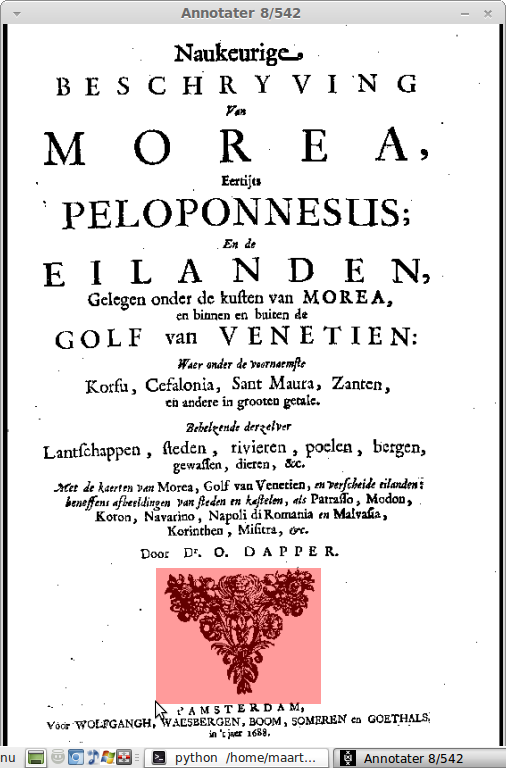
\includegraphics[width=\textwidth]{resources/screenshotAnnotator}
    \caption{A screen shot of the Annotator tool with an image in a bounding box}
    \label{fig:ann}
\end{wrapfigure}

An annotator was built, in order to quickly and easily annotate all the pages of
a book. When a book is downloaded, the annotator cycles through all its pages.
The user can then press a button on the keyboard indicating whether the page
contains an image, text, or neither. When the page contains one or several
images, the user has to drag a bounding box around the images, using the mouse,
prior to pressing the keyboard button. Errors can be reversed if a page was
skipped too quickly, or if the user felt a bounding box was drawn incorrectly.
Because the majority of the pages are
text pages and the user only has to press 1 button per page, books can be
annotated fairly quickly with this tool.

Using this annotator and the Google Books website, a training set of annotated
book pages was created, containing 5960 pages from 23 books. The statistics of
this dataset can be seen in table \ref{tab:statistics}. A separate test set
containing 2868 pages from 4 books was created as well. Both sets can be
requested via E-mail.



